%----------------------------------------------------------
\chapter{Классификация систем типов}
\label{ch:classification}
%----------------------------------------------------------

Известно, что системы типов можно разделить на \textit{динамические} и \textit{статические} \cite{Typing}.
Это влияет на то, в какой момент в программе происходит проверка соответствия типов.
В динамических системах - во время исполнения программы, а в статических - соответственно во время компиляции.
Кроме того, существуют особые языки программирования, где в сущности все является одним типом.
К таким относится ассемблер: все - набор битов, и нетипизированное \gls{LC}, где все есть функция.

Далее будут рассмотрены только статические системы типов, так как после семантического анализа, компилятор может использовать накопленную информацию для оптимизации кода.
Это делает языки со статической типизацией, хоть и более сложными в использовании, но более быстрыми, а динамически типизированным языкам приходится использовать различные специфические оптимизации, например, JIT-компиляцию, чтобы добиться сопоставимой скорости.

Ниже приведены основные критерии, по которым можно классифицировать языки программирования:

\begin{enumerate}
    \item по времени проверки соответствия типам:
    \begin{itemize}
        \item статическая,
        \item динамическая;
    \end{itemize}
    \item по поддержке неявных конверсий:
    \begin{itemize}
        \item сильная,
        \item слабая;
    \end{itemize}
    \item по необходимости вручную типизировать выражение:
    \begin{itemize}
        \item явная,
        \item неявная;
    \end{itemize}
\end{enumerate}

Предлагается исследовать существующие решения среди различных языков программирования и выделить в них положительные и отрицательные стороны.

\section{Система типов C}
\label{sec:c_type_system}

Типом в языке C является интерпретация набора байт, составляющих объект.
Такой подход характерен для довольно низкоуровневых языков.

Все типы делятся на две группы:
\begin{itemize}
    \item скалярные - в них входят примитивные (базовые) типы, которые описывают множество различных вариантов представления числа, а также указатели,
    \item агрегатные - определяемые пользователем структуры, состоящие из упорядоченного именованного набора других типов, и массивы какого-то конкретного типа;
\end{itemize}

Кроме того, существуют <<специальные>> типы - объединения и функции.
Специальные они потому что в первом случае - это лишь особый вариант структуры, а во втором - существуют только указатели на функции: отдельного типа для лямбда-фукнции в C нет.

\textbf{Достоинства:}
\begin{itemize}
    \item Си прост для понимания, он содержит только основные типы данных,
    \item язык позволяет эффективно работать с данными в том виде, как они реализованы в ЭВМ.
\end{itemize}

\textbf{Недостатки:}
\begin{itemize}
    \item недостаточная экспрессивность по сравнению с другими языками программирования,
    \item мало гарантий и проверок, осуществляемых компилятором.
\end{itemize}

\section{Система типов Kotlin}
\label{sec:kotlin_type_system}

Пару слов о языке: разрабатывается компанией JetBrains с 2011 года, работает на платформе \gls{JVM} (хотя поддерживает и другие).
Популярен среди приложений под ОС Android\cite{KotlinTypeSpec}.

\textbf{Достоинства:}
\begin{itemize}
    \item имеет более продвинутую, по сравнению с Java, систему типов, включающую \textit{nullable types} и ограниченно типы-произведения,
    \item хороша для описания классов в виде, привычном в \gls{OOP}.
\end{itemize}

\textbf{Недостатки:}
\begin{itemize}
    \item из-за специфики работы обобщенных типов в \gls{JVM}\footnote{см. type erasure} иногда довольно сложно узнать, какой тип был изначально,
    \item все еще менее выразительна, по сравнению с некоторыми функциональными языками
\end{itemize}

\section{Система типов ML-подобных языков}
\label{sec:ml_type_system}

В основе системы типов типизированных функциональных языков, таких как ML или Haskell, лежит \gls{TLC}.
Это формализованная система для описания программ, предложенная Алонзо Чёрчем в 1930 году.

Кроме проверки типов, над такими системами можно удобно проводить \textit{вывод типов}.
Это позволяет пользователю составлять программы почти не используя аннотации типов.

\subsection{Лямбда-куб}
\label{subsec:lambda_cube}

Эта абстракция позволяет наглядно увидеть разницу и взаимоотношение между различными видами \gls{TLC} (см. рис. \ref{fig:lambda_cube}).

\begin{figure}[H]
    \centering
    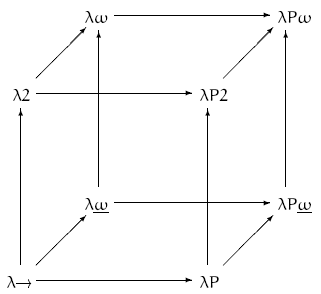
\includegraphics[width=0.45\textwidth]{figures/Lambda_cube}
    \caption{Графическое изображение лямбда-куба}
    \label{fig:lambda_cube}
\end{figure}

Простейшим вариантом является \textit{просто типизированное лямбда-исчисление} ($\lambda \to$).
В нем доступна абстракция только с помощью функции:

\begin{equation}
    \label{eq:STLC}
    \frac{\Gamma \cup x: T \vdash y: U}{\Gamma \vdash \lambda x.y: T \to U}
\end{equation}

Следующим этапом является \textit{полиморфное лямбда-исчисление} ($\lambda 2$).
В нём термы могут зависеть от типов (обобщенные функции):

\begin{equation}
    \label{eq:2TLC}
    \frac{\Gamma \vdash y: U}{\Gamma \vdash \forall T: \lambda (x: T).y: T \to U}
\end{equation}

Еще одним расширением будет \textit{лямбда-исчисление с операторами над типами} ($\lambda \underline{w}$).
С точки зрения обычных языков программирования такое исчисление формирует функции над типами:
В частности, функция, формирующая тип списка, выглядела бы так:

\begin{equation}
    \label{eq:WTLC}
    \lambda \alpha: *. \alpha \to List ~\alpha
\end{equation}, где $*$ - любой другой тип

Последней простой точкой куба является \textit{лямбда-исчисление с зависимыми типами} ($\lambda P$).
Оно примечательно тем, что типы могут зависеть от термов.
Наиболее простым примером послужит функция деления, где входной аргумент обязан быть отличным от $0$.

Остальные вершины являются комбинацией описанных систем.

Подведем итог.

\textbf{Достоинства:}
\begin{itemize}
    \item выразительность системы типов легко показать том же самом лямбда-кубе,
    \item имеет строгое математическое обоснование и хорошо изучено,
    \item компилятор имеет возможность выявить больше ошибок в программе.
\end{itemize}

\textbf{Недостатки:}
\begin{itemize}
    \item достаточно сложна для понимания как с точки зрения пользователя, так и разработчика компилятора
    \item может значительно увеличить время компиляции
\end{itemize}

%----------------------------------------------------------
